

\section{Introduction}

\label{sect:introduction}

Much of computer vision is passive in nature, with the emphasis on
watching the world but not participating in it.  There are advantages
to moving beyond this to exploit dynamic regularities of the
environment \cite{ballard91animate}.
%%,breazeal00social}.  
A robot has the
potential to examine its world using causality, by performing probing
actions and learning from the response.  Tracing chains of causality
from motor action to perception (and back again) is important both to
understand how the brain deals with sensorimotor coordination and to
implement those same functions in an artificial system, such as a
humanoid robot.  And, as a practical matter, the ability to perform
``controlled experiments'', such as tapping an object lightly, is
crucial to getting to grips with an otherwise complex and uncertain
world.

\ifverbose
In the context of sensorimotor coordination causality can be operationally
defined as a functional link between some variables, being these motor,
sensorial, or both.  At higher levels of abstaction other quantities might
need to be considered, not necessarily, purely sensorial or motor but
rather combinations of various sort. Causality accounts to discovering
similarity and recurrence in this sensorimotor data, possibly delayed of
unknown amounts.
\fi


Figure~\ref{fig:tracing-causes} shows three levels of causal complexity
we would like the robot to probe.
The simplest causal chain that the robot experiences is the
perception of its own actions.  The temporal aspect is immediate:
visual information is tightly synchronized to motor commands.
We use this strong correlation to identify parts of the robot
body -- specifically, the end-point of the arm. 

Once this causal connection is established, we can go further and use
it to actively explore the boundaries of objects.  In this case, there
is one more step in the causal chain, and the temporal nature of
the response may be delayed since initiating a reaching movement doesn't
immediately elicit consequences in the environment.  

\ifverbose
relation and a
more subtle perception of space has also to be taken into account, e.g
localization of the effector, and the spatial relation with the
manipulated object.  The temporal aspect in this case assumes a
delayed form: triggering a reaching movement doesn't immediately
elicit consequences in the environment.

We
show how an active exploration strategy might explain how newborns
develop, during ontogenesis, figure-ground segregation capabilities.
The temporal aspect in this case assumes a delayed form: triggering a
reaching movement doesn't automatically elicit consequences in the
environment. Towards reaching completion a more immediate form can
take place due to correlation between the haptic and visual responses.
\fi


In this paper, we propose that such causal probing can be arranged in
a developmental sequence leading to a manipulation-driven
representation of objects.  We present results for two important
steps along the way, and describe how we plan to proceed.
We argue that following this causal chain outwards will allow
us to approach the representational power of ``mirror
neurons'' \cite{fadiga00visuomotor}, where a connection is made
between our own actions and the actions of another.

\ifverbose
The third case is a more conceptual one and it represents our more long
term goal in terms of robotic implementation. It is interesting though
because it can be explained by the same principle of causality. This
is the case of ``mirror neurons'' \cite{fadiga00visuomotor}. The
details of this third example are presented later.  Development takes
an even more delayed form involving probably a form of long-term
memory. Our everyday personal experience on the manipulation of objects is
reused to interpret the same class of manipulative acts when performed
by somebody else.  Clearly the two situations, when acting and when watching,
 are not necessarily simultaneous.
\fi

\ifverbose
This solves a problem,
difficult if addressed visually, by taking advantage of the fact the
system is embodied.  There are examples of similar behaviors in
newborns [I still have to find the refs in this case]. The level of
causality exploited here is a direct one. 
\fi

\ifverbose
  Of
course, processing delays must be accounted for -- in the brain,
delays are known to depend on the modality (e.g. vision is slower than
for example vestibular signals) and consequently multisensory or
sensorimotor integration has to compensate for them.
\fi



\ifverbose
There is a bulk of neuroscience data on all this aspect of human
sensorimotor cognition. For the purpose of this paper, we first would
like to show that there is indeed a problem if the agent is not
properly situated[? does it make any sense ?]. A nice example is the
definition of ``object''.  We will devote a
section to illustrate this point which turns out to be central in a
series of tasks including the three cases analyzed before. Many of our everyday's
acts are definitely object-oriented.

Developmentally we can explain what is an ``object'' by exploiting
the fact that the agent is embodied.
By looking at the three examples, we can notice a trend in complexity, 
and consequently we can hypothesize, that the time required to reach proficiency 
in each task is proportional to this complexity. Table~\ref{tab:causation} shows this idea.
\fi

\ifverbose
\begin{table*}[htbp]
\begin{center}
\begin{tabular}{|p{4.8cm}|p{4.8cm}|p{4.8cm}|}
\hline
{\it type} & {\it nature of causation} &  {\it time profile} \\ \hline\hline
{\bf sensorimotor coordination} & direct causal chain & strict synchrony \\ \hline
{\bf object probing} & one level of indirection & fast onset upon contact, potential for delayed effects\\ \hline
{\bf mirror representation} &  complex causation involving multiple causal chains & arbitrarily delayed onset and effects\\ \hline
\end{tabular}
\caption{
\label{tab:causation}
%
Degrees of causal indirection. There is a natural
trend from simpler to more complicated tasks.  The more time-delayed
an effect, the more difficult it is to model.
%
}
\end{center}
\end{table*}
\fi

%
\begin{figure}[tb]
\begin{center}
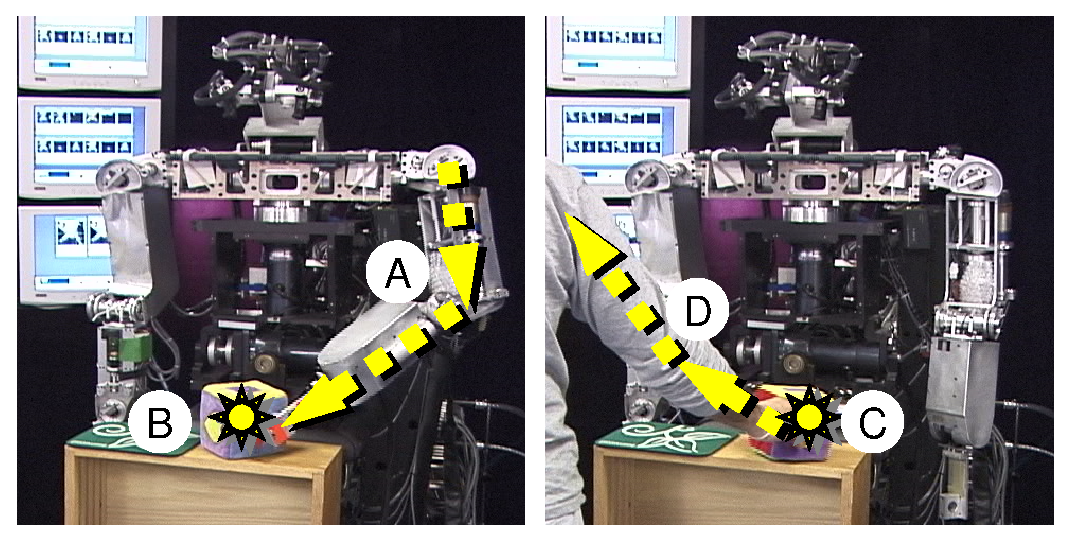
\includegraphics[width=\columnwidth]{tracing_causes.eps}
\caption{ 
\label{fig:tracing-causes}
%
On the left, the robot establishes a causal connection between
commanded motion and its own manipulator (A), and then probes its
manipulator's effect on an object (B).  The object then serves as a
literal ``point of contact'' (C) to link robot manipulation with human
manipulation (on the right, D), as is required for a mirror-neuron-like
representation.
%
}
\end{center}
\end{figure}
%



\ifverbose
The more strict
temporal aspect on the other hand require perfect timing (within the
bandwidth of the process considered of course), but the cause-effect
linkage is a direct one.
For the purposes of manipulation, we would like to know what parts of
the environment are physically coherent ensembles -- that is, which
parts will move together, and which are more or less independent.  It
takes a great deal of experience before this judgement can be made
from purely visual information.  This paper develops active strategies
for acquiring that experience through experimental manipulation, using
tight correlations between arm motion and optic flow to detect both
the arm itself and the boundaries of objects with which it comes into
contact.
\fi




\section{The elusive object}


Sensory information is intrinsically ambiguous, and very distant from
the world of well-defined objects in which humans believe they live.  
What criterion should be applied to distinguish one object from
another?  How can perception support such a phenomenon as figure-ground
segmentation?  
Consider the example in Figure~\ref{fig:number-cross}.  It is
immediately clear that the drawing on the left is a cross, perhaps
because we already have a criterion, which allows segmenting on the
basis of the intensity difference. It is slightly less clear that the
zeros and ones on the middle panel are still a cross. What can we say
about the array on the right? If we are not told, and we do not have
the criterion to perform the figure-ground segmentation, we might
think this is just a random collection of numbers. But if we are told
that the criterion is ``prime numbers vs. non-prime'' then a cross can
still be identified.

While we have to be inventive to come up with a segmentation problem
that tests a human, we don't have to go far at all to find something
that baffles our robots.  Figure~\ref{fig:setup-sequence} shows a
robot's-eye view of a cube sitting on a table.  Simple enough, but
many rules of thumb used in segmentation fail in this particular case.
And even an experienced human observer, diagnosing the cube as a
separate object based on its shadow and subtle differences in the
surface texture of the cube and table, could in fact be mistaken --
perhaps some malicious researcher is up to mischief.  The only way to
find out for sure is to take action, and start poking and prodding.
As early as 1734, Berkeley observed that:
%
\begin{quote}
...objects can only be known by
touch. Vision is subject to illusions, which arise from the
distance-size problem... \cite{berkeley72new}
\end{quote}
%
In this paper, we provide support for a more nuanced proposition: that
in the presence of manipulation, vision becomes more powerful, and many of
its illusions fade away.


%
\begin{figure}[tb]
\begin{center}
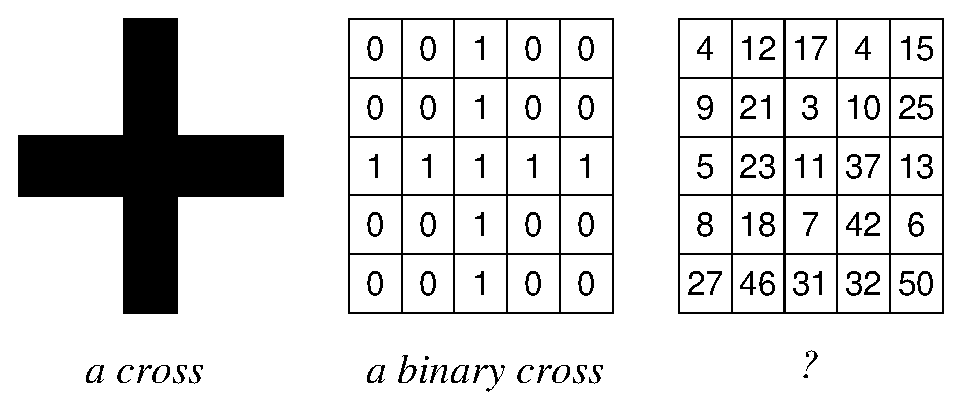
\includegraphics[width=6.5cm]{number-cross.eps}
\caption{ 
\label{fig:number-cross}
%
Three examples of crosses, following \cite{manzotti01coscienza}.  The
human ability to segment objects is not general-purpose, and improves
with experience.
%
}
\end{center}
\end{figure}
%
%
\begin{figure}[tb]
\begin{center}
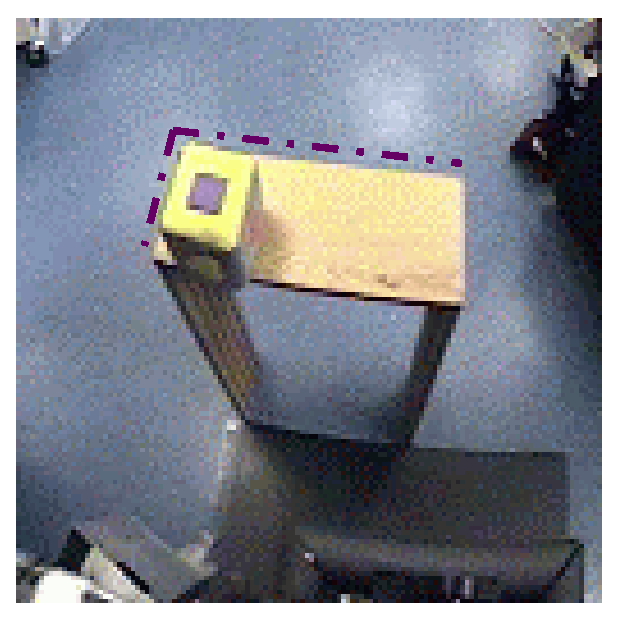
\includegraphics[width=4cm]{setup-sequence.eps}
%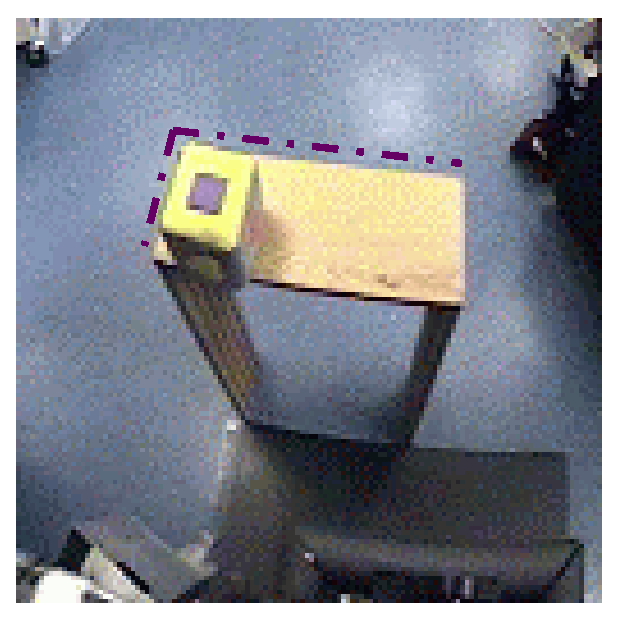
\includegraphics[width=\columnwidth]{setup-sequence.eps}
%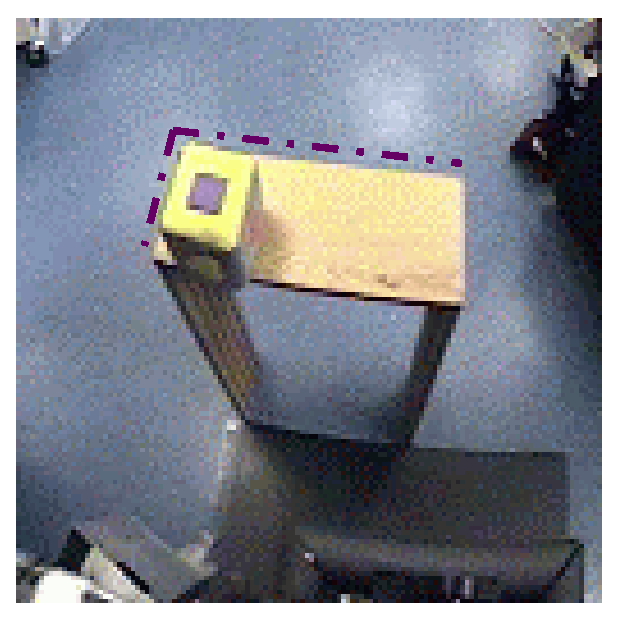
\psfig{file=setup-sequence.eps,width=4cm}
\caption{ 
\label{fig:setup-sequence}
%
A cube on a table. The edges of the table and cube happen to be
aligned (dashed line), the colors of the cube and table are not well
separated, and the cube has a potentially confusing surface pattern.
%
}
\end{center}
\end{figure}

\subsubsection*{Objects and actions}

The example of the cross composed of prime numbers is a novel (albeit
unlikely) type of segmentation in our experience as adult humans. We
might imagine that in our infancy, we had to initially form a set of
criteria to solve the object identification/segmentation problem
in more mundane circumstances.  We ask the question of whether we can
discover these criteria during ontogenesis.

Humans and a small number of other primates are unique in their
ability to manipulate their environment using tools.
Our capacities are mirrored in the brain by the size of
the cortex controlling them.  Neuroscience has shown that our brains
possess large cortical areas devoted to the control of manipulation --
not surprising, given that encephalization is believed to have evolved
for the purpose of adaptively controlling
action \cite{maturana98tree}.

A useful conceptual schema holds that visual information follows two
distinct pathways in the brain, namely, the dorsal and the ventral
\cite{ungerleider82two,milner95visual}.
The dorsal
pathway controls action directly and pragmatically; conversely, the
ventral takes care of more conceptual skills such as object
recognition.
Of course it is important to remember, when making this dichotomy,
that the two pathways are not completely segregated but rather
complement each other and interact in different
ways \cite{jeannerod97cognitive}.

%%This concept of two distinct visual systems was initially proposed by
%%\cite{ungerleider82two}
%%and successively
%%refined by 
%%Milner and Goodale
%%\cite{milner95visual}. 

Objects are thought to maintain a double ``identity'' depending on
whether they are used in perceptual or in motor tasks. The concept of
size, for example, might be represented multiple times in different
brain areas. Observation of agnosic
patients \cite{jeannerod97cognitive} shows an even more complicated
relationship than the simple dorsal/ventral dichotomy would
suggest.  Althought some patients could not grasp generic objects
(e.g. cylinders), they could correctly preshape the hand to grasp
known objects (e.g. a lipstick); interpreted in terms of the
two-pathway system, this implies that the ventral representation of
the object can supply the dorsal system with size information. What we
consciously perceive as ``size'' is rather a collection of different
percepts interacting in a complicated way, and under pathological
circumstances they can be separated from each other. One of the
``identities'' of objects is thus connected to motor performance.

That such pathways develop and are not completely innate is suggested
by the results of \cite{kovacs00human}. She has shown that
perceptual grouping is slow to develop and continues to improve well
beyond early childhood (14 years). Long-range contour integration was
tested and this work elucidated how this ability develops to enable
extended spatial grouping. These results further suggest that the
development of action might precede that of categorization: it is well
enstablished that by 4 months of age infants can process complex
motion stimuli, depth, and color.  Roughly at the same age reaching
becomes more consistent.  That is, action comes first
supported by the pragmatic use of diverse sensory modalities;
perception conversely is a long developing process. More studies are
needed though to ascertain how the dorsal pathway (action) influences
the ventral (perception) both in situations like those
already mentioned, and during ontogenesis.

The dorsal stream connects the parietal lobe to the premotor cortex,
which project heavily onto the primary motor cortex to eventually
control movements.  For many years the premotor cortex was considered
just another big motor area.  New studies
\cite{jeannerod97cognitive} have demonstrated that this is not the
case.  In fact, researchers have identified neurons in the area F5 of
the frontal cortex \cite{fadiga00visuomotor} that are activated in two
situations: {\it i)} when acting onto an object (e.g. grasping), and
{\it ii)} when looking at the same object (visual response). Their
firing pattern was quite specific, building a link between the size of
the object and the applied grasp type (e.g. a small object requires a
precision grip).
 
These neurons were called canonical. This was quite an astonishing
discovery because area F5 was believed to be only a motor area. A
possible interpretation is that the brain stores a representation of
objects in motor terms, and uses these representations to generate an
appropriate response to objects (the concept of Gibsonian affordances
translated in neural terms \cite{gibson77theory}).

The gap from object manipulation to hand gesture
production/recognition is small.  In fact F5 contains another class of
neurons called mirror neurons. A mirror neuron responds in two
situations: {\it i)} when executing a manipulative gesture, and {\it
ii)} when observing somebody else executing the same action. These
neurons provide a link between the observation of somebody else's
and our own actions.  Beside the recognition of manipulative actions,
they seem to support imitative behaviors. An intriguing theory
proposed by Rizzolatti and Arbib \cite{rizzolatti98language}
associates mirror neurons to language.
%% and to the motor theory of language.

\ifverbose
The dorsal/ventral dichotomy is of course a gross simplification of
the reality.  There are neurons in area STS (superior temporal sulcus,
which is a ventral area) that respond to the sight and specific
posture of the hand. They are quasi-mirror neurons but they lack the
motor component (they do not fire in the dark).  Area STS is supposed
to provide the visual information about the posture of the hand to F5
[CITE].
\fi

Another important class of neurons in premotor cortex is found in area
F4 \cite{fogassi96coding}. While F5 is more concerned with the distal
muscles (i.e. the hand), F4 controls more proximal muscles
(i.e. reaching). A subset of neurons in F4 has a somatosensory, visual
and motor receptive field. The visual receptive field (RF) extends in
3D from a given body part, for example, the forearm. The somatosensory
RF is usually in register with the visual one. Finally, motor
information is integrated into the representation by maintaining the
RF anchored to the correspondent body part (the forearm in this
example) irrespective of the relative position of the head and arm.


\subsubsection*{A working hypothesis}

In the light of these results, we see at least two reasons why
intelligence needs to be embodied. First, if robots are to tell us
something about the functioning of our brains, we have to study its
development in the proper setting, that is, with the robot acting in
the environment. As we have seen action is fundamental to a set of
highly cognitive skills including imitation and language. Perceptual
tasks are also be influenced by action. Second, to build better
robots, adaptive to their environment, there is probably no
alternative but to build them following to some extent biological
principles. The same constraints encountered by biological agents
during ontogenesis are encountered by the robot during its simulated
development.

Certainly, vision and action are intertwined at a very basic level.
While an
experienced adult can interpret visual scenes perfectly well without
acting upon them, linking action and perception seems crucial to the
developmental process that leads to that competence.  We can construct
a working hypothesis: that action is required to object recognition in
cases where an agent has to develop categorization autonomously.  Of
course in standard supervised learning action is not required since
the trainer does the job of pre-segmenting the data by hand.  In an
ecological context, some other mechanism has to be provided.
Ultimately this mechanism is the body itself that through action
(under some suitable developmental rule) generates informative
percepts.

Neurons in area F4 are thought to provide a body map useful for
generating arm, head, and trunk movements. Our robot learns
autonomously a crude version of this body map by fusing vision and
proprioception.  As a step towards establishing the kind of visuomotor
representations seen in F5, we then develop a mechanism for using
reaching actions to visually probe the connectivity and physical
extent of objects without any prior knowledge of the appearance of the
objects (or indeed of the arm itself).


\ifverbose

[1] \cite{maturana98tree}
[2] \cite{milner95visual}
[3] \cite{jeannerod97cognitive}
[4] \cite{konczak}
[5] \cite{fadiga00visuomotor}
[6] \cite{gibson77theory}
[7] \cite{rizzolatti98language}


[1]
Maturana, R.H. and F.J. Varela, 
The tree of knowledge, the biological roots of human understanding. 
Revised Edition ed. 1998, Boston & London: Shambhala Publications, Inc. 269.

[2]
Milner, D.A. and M.A. Goodale, 
The Visual Brain in Action. Oxford Psychology. Vol. 27. 1995, 
Oxford: Oxford University Press.

[3]
Jeannerod, M., 
The Cognitive Neuroscience of Action. Fundamentals of Cognitive Neuroscience, 
ed. M.J. Farah and M.H. Johnson. 1997, Cambrige, MA and Oxford UK: 
Blackwell Publishers Inc. 236.

[4]
Konczak, J.,
///

[5]
Fadiga, L., et al., Visuomotor neurons: ambiguity of the discharge of 
'motor' perception? Internation Journal of Psychophysiology, 2000. 35(2-3): p. 165-177.

[6]
Gibson, J.J., 
The theory of affordances, in Perceiving, acting and knowing: toward an 
ecological psychology, R. Shaw and J. Bransford, Editors. 1977, 
Lawrence Erlbaum: Hillsdale. p. 67-82.

[7]
Rizzolatti, G. and M.A. Arbib, 
Language within our grasp. Trends in Neurosciences, 1998. 21(5): p. 188-194


\fi